\section{Analysis of type systems}



\begin{table*}[htbp]
    \caption{Several type systems of MPLs}
    \label{tab:type}
    \begin{center}
        \begin{tabular}{cccccc}
            \toprule
            Language & Typed/Untyped & Explicitly/Implicitly typed &
            Dynamically/Statically checked & Strongly/Weakly checked & Well behaved\\
            \midrule
            Python     & Typed   & Implicitly & Dynamically & Strongly & Yes \\
            Java       & Typed   & Explicitly & Statically  & Strongly & Yes \\
            C++        & Typed   & Explicitly & Statically  & Weakly   & No  \\
            JavaScript & Untyped & -          & Dynamically & -        & Yes \\
            Go         & Typed   & Explicitly & Statically  & Strongly & Yes \\
            Swift      & Typed   & Explicitly & Statically  & Strongly & Yes \\
            Dart       & Typed   & Explicitly & Statically  & Strongly & Yes \\
            Rust       & Typed   & Explicitly & Statically  & Strongly & Yes \\
            Kotlin     & Typed   & Explicitly & Statically  & Strongly & Yes \\
            \bottomrule
        \end{tabular}
    \end{center}
\end{table*}


The discussion here is based on L. Cardelli's definition of type systems\cite{cardelli1996type}.
L. Cardelli considers that the fundamental purpose of
type systems of a languages is to prevent errors that occur during the runtime,
so he discusses type systems by defining concepts related to errors.
According to Figure~\ref{fig:type-definition}, there are two types of errors.
An error that immediately results in a fault is called a trapped error.
The other will not cause fault immediately, called untrapped error.
All untrapped errors and some trapped errors are collectively
called forbidden errors.

\begin{figure}[htbp]
    \centerline{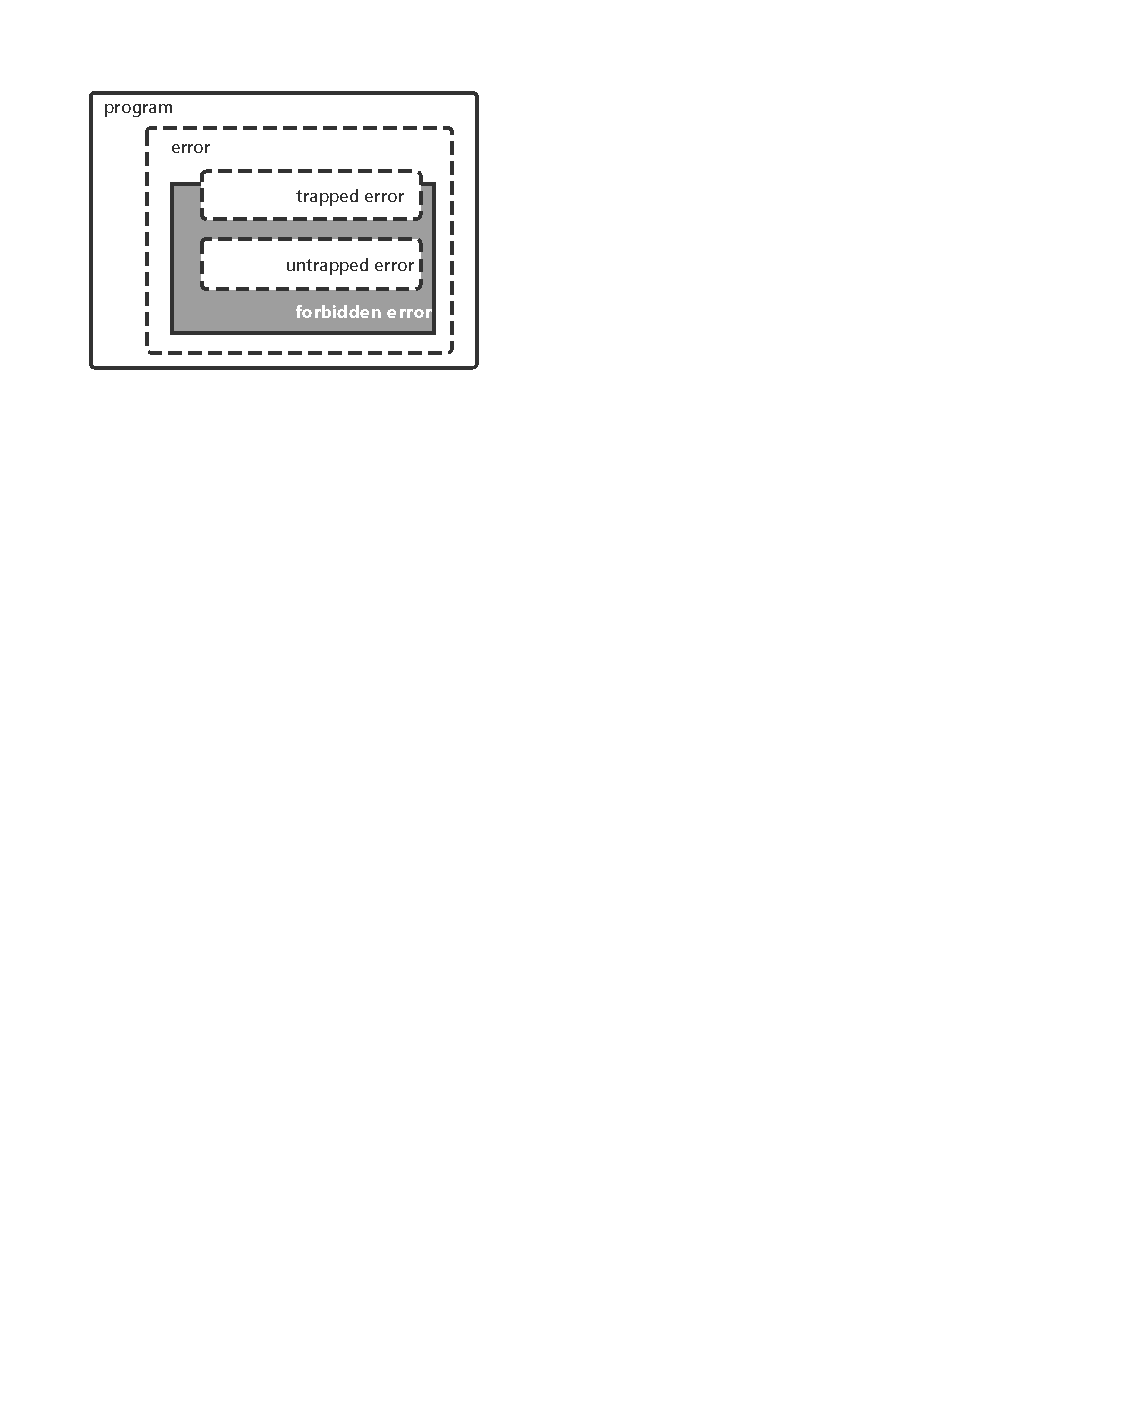
\includegraphics[scale=0.8]{figures/type-definition}}
    \caption{Definition of forbidden error}
    \label{fig:type-definition}
\end{figure}


programming languages are divided into (statically) typed languages and (statically) untyped languages
depending on whether they have static types to limit the scope of variable types at runtime.
Based on the timing of behavior checking, programming languages
can be classified as statically checked languages and dynamically checked languages.
Based on statically checked languages, languages that cannot find out all forbidden
errors are called weakly checked languages.
Conversely, languages that find out all forbidden errors are called strongly checked languages.
Then explicitly typed languages and implicitly typed languages are
classified according to whether the programming language explicitly
specifies the type of the variable.
A program is said to have good behavior if it does not produce
forbidden errors during execution.
According to the above definition,
we have analyzed 9 selected languages and got the Table~\ref{tab:type}.

There is one thing to note.
Type hints were introduced in Python in version 3.5.
But type hints do not actually do error checking for Python.
It is simply a type annotation to help provide better support
for static analysis of syntax parsers.
The real time for error checking is still at runtime.
So Python is still a dynamically checked, strongly checked language.

Table~\ref{tab:type} gives the type system of common MPLs according
to L. Cardelli's type system definition.
It is worth noting that most current MPLs have certain commonalities.
They are often explicitly typed, strongly checked, statically checked, and well-behaved.
This is inseparable from the application scenarios of these languages.
Type signatures contain constraint information by which the behavior of
variables or functions can be indirectly determined.
It also improves maintainability, which is exactly what programming languages
for industrial applications need.
Static type checking and formal proofs of type systems improve the reliability
of programs and help people write less error-prone code.
Also, a static type system is more conducive to performance optimization
and memory allocation, and object programs after compilation can have better performance.
